\chapter[ಅಧ್ಯಾಯ 2]{}\label{chap2}

\begin{center}
\rule{5cm}{1pt}\\[5pt]
{\Large\bfseries ಸಮಸ್ಯೆಗಳು}\\[3pt]
\rule{5cm}{1pt}
\end{center}

\smallskip
\begin{enumerate}
\renewcommand{\labelenumi}{\bf\theenumi.}
\itemsep=5pt
\item ನಾಲ್ಕು 4 ಬಳಸಿ 1 ರಿಂದ 10 ರವರೆಗೆ ಬರಿಸಿ. ಯಾವುದೇ ಗಣತೀಯ ಚಿಹ್ನೆ, ಪ್ರಕ್ರಿಯೆ ಬಳಸಬಹುದು.

\item 0, 1, 2, 3, 4, 5, 6, 7, 8, 9 ಈ ಅಂಶಗಳನ್ನೆಲ್ಲ ಒಮ್ಮೆ ಮಾತ್ರ ಬಳಸಿ, 9 ಬರಿಸಿ. ಯಾವುದೇ ಗಣಿತೀಯ ಚಿಹ್ನೆ, ಪ್ರಕ್ರಿಯೆ ಬಳಸಬಹುದು. 

\item 987654321 ಅಂಕಿಗಳ ಕ್ರಮ ಬದಲಿಸದೆ, $+/-$ ಚಿಹ್ನೆ ಬಳಸಿ 100 ಬರಿಸಿ.

\item ಐದು ಬೆಸ ಸಂಖ್ಯೆಗಳ ಮೊತ್ತ 20 ಆಗುವಂತೆ ಮಾಡಿ. ಬಳಸಿದ ಸಂಖ್ಯೆಯನ್ನೇ ಮತ್ತೆ ಬಳಸಬಹುದು. 

\item 1, 2, 3, 4, 5, 6, 7, 8, 9 - ಇವುಗಳನ್ನು 2 ಗುಂಪುಮಾಡಿ. ಪ್ರತಿ ಗುಂಪಿನ ಅಂಕಿಗಳಿಂದ ಎರಡೆರಡು ಸಂಖ್ಯೆ ರಚಿಸಿ. ಸಂಖ್ಯೆಗಳ ಮೊತ್ತ ಸಮವಾಗಬೇಕು. 

\item ಮೂರು 8ಗಳನ್ನು ಯಾವುದೇ ಗಣಿತ ಚಿಹ್ನೆ, ಪ್ರಕ್ರಿಯೆಗಳಿಂದ ಜೋಡಿಸಿ 7 ಉತ್ತರ ಬರಿಸಿ.

\item XVII ಇದನ್ನು ಪುನರ್ಜೋಡಿಸಿ 100 ಬರಿಸಿ.

\item LXVIII ಗೆರಗಳನ್ನು ಪುನರ್ಜೋಡಿಸಿ 10 ಬರಿಸಿ. 

\item IV = III $-$ I ಒಂದು ಅಥವಾ 2 ಗೆರೆ ಸ್ಥಾನ ಪಲ್ಲಟ ಮಾಡಿ ಸಮೀಕರಣ ಸರಿದೂಗಿಸಿ $\neq$ ಬರುವಂತಿಲ್ಲ.

\item $\frac{XXII}{VIII} = II$ ಪುನರ್ಜೋಡಿಸಿ, ಸಮೀಕರಣ ಸರಿದೂಗಿಸಿ $\neq$ ಬರುವಂತಿಲ್ಲ.

\item $\frac{I}{VII} = I$ ಪುನರ್ಜೋಡಿಸಿ, ಸಮೀಕರಣ ಸರಿದೂಗಿಸಿ $\neq$ ಬರುವಂತಿಲ್ಲ

\item 24 ಬೆಂಕಿಕಡ್ಡಿಗಳಿಂದ 3 $\times$ 3 ಚೌಕ ರಚಿಸಿದೆ.

\begin{minipage}[c]{5cm}
\begin{tabular}[t]{ll}
ಇದರಲ್ಲಿ  & \\
1 ಕಡ್ಡಿ ಅಳತೆಯ  & 9 ಚೌಕಗಳು \\
2 ಕಡ್ಡಿ ಅಳತೆಯ & 4 ಚೌಕಗಳು\\
3 ಕಡ್ಡಿ ಅಳತೆಯ & 1 ಚೌಕ\\
\hline
\qquad ಒಟ್ಟು & 14 ಚೌಕಗಳು ಇವೆ.\\
\hline
\end{tabular}
\end{minipage}
\begin{minipage}[c]{4cm}
\begin{figure}[H]
\centering
\includegraphics{images/chap2/q12.eps}
\end{figure}
\end{minipage}

\medskip

ಚೌಕಗಳೇ ಇಲ್ಲದಂತೆ ಮಾಡಲು ಕನಿಷ್ಠ ಎಷ್ಟು ಕಡ್ಡಿ ತೆಗೆಯಬೇಕು? 

\item 12 ಬೆಂಕಿಕಡ್ಡಿಗಳ ಜೋಡಣೆ ಹೀಗಿದೆ ಯಾವುದಾದರೂ 3 ಕಡ್ಡಿ ಸ್ಥಾನ ಪಲ್ಲಟ ಮಾಡಿ 5 ಚೌಕ ಬರಿಸಿ. 
\begin{figure}[H]
\centering
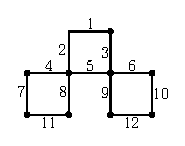
\includegraphics{images/chap2/q13.eps}
\end{figure}

\item 8 ಬೆಂಕಿಕಡ್ಡಿ ಜೋಡಿಸಿ 2 ಚೌಕಗಳು, 8 ತ್ರಿಭುಜಗಳು, 1 ಬಹು ಭುಜಾಕೃತಿ ಬರಿಸಿ. 

\item 3 ಬೆಂಕಿಕಡ್ಡಿಗಳಿಂದ ರಚಿಸಬಹುದಾದ ಅತಿ ದೊಡ್ಡ ಸಂಖ್ಯೆ ಯಾವುದು? 

\item 13 ಬೆಂಕಿಕಡ್ಡಿಗಳ ಜೋಡಣೆ ಹೀಗಿದೆ. ಯಾವ 3 ಕಡ್ಡಿ ತೆಗೆದರೆ ತ್ರಿಭುಜಗಳು ಮಾತ್ರ ಉಳಿಯುತ್ತವೆ? 

\begin{figure}[H]
\centering
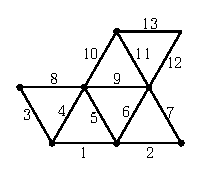
\includegraphics{images/chap2/q16.eps}
\end{figure}

\eject

\item ಈ ಗುಣಾಕಾರವನ್ನು ಅಭ್ಯಸಿಸಿ. 
\begin{align*}
6 \times 6 & = 36\\
66 \times 66 & = 4356\\
666 \times 666 & = 443556\\
6666 \times 6666 & = 44435556\\
\end{align*}

ಮುಂದಿನ 4 ಲಬ್ಧಗಳನ್ನು ಬರೆಯಿರಿ. 

\item 333333666667 $\times$ 33 = 11000011000011 ಗುಣಲಬ್ಧ ಮಾಲಾ ಸಂಖ್ಯೆ (Palindrome number). ಯಾವ ಕಡೆಯಿಂದ ಓದಿದರೂ ಅದೇ ಗಣಿತಜ್ಞ ವರಾಹರಿಹಿದಾಚಾರ್ಯರ “ಗಣಿತ ಸಾರಸಂಗ್ರಹ" ಗ್ರಂಥದಲ್ಲಿ ಇನ್ನೂ ಅನೇಕ ಉದಾಹರಣೆಗಳಿವೆ.

\item 142857 ಇದೊಂದು ವಿಶಿಷ್ಟ ಸಂಖ್ಯೆ ಅದನ್ನು 2, 3, 4, 5, 6 ರಿಂದ ಗುಣಿಸಿ

\begin{minipage}[c]{5cm}
\begin{tabular}{ll}
$142857 \times 2$ & = $287514$\\
$142857 \times 3$ & = $428751$\\
$142857 \times 4$ & = $571428$\\
$142857 \times 5$ & = $714285$\\
$142857 \times 6$ & = $857142$
\end{tabular}
\end{minipage}
\begin{minipage}[c]{4cm}
\begin{figure}[H]
\centering
\includegraphics{images/chap2/q19.eps}
\end{figure}
\end{minipage}

ಲಬ್ಧದಲ್ಲಿ 6ನೇ 6 ಅಂಕಿಗಳಿವೆ. ಚಕ್ರೀಯ ಕ್ರಮದಲ್ಲಿ ಬರುತ್ತದೆ. ಇಂತಹ ಸಂಖ್ಯೆಗೆ ಚಕ್ರೀಯ ಸಂಖ್ಯೆ (Cyclic number) ಎಂದು ಹೆಸರು. 

7 ರಿಂದ ಗುಣಿಸಿದಾಗ 999999 ಲಭ್ಯ

\item ಈ ಆಕೃತಿಯಲ್ಲಿರುವ ಚೌಕಗಳೆಷ್ಟು?
\begin{figure}[H]
\centering
\includegraphics{images/chap2/q20.eps}
\end{figure}
 
\item ಘನಾಕೃತಿ (cube) ಅತಿ ಉತ್ಕೃಷ್ಟ ಎಂದ ಪ್ಲೇಟೊ ಆತನ ಒಂದು ಸಮಸ್ಯೆ - ಗಾತ್ರದ ಅಳತೆಯಷ್ಟೇ ಮೇಲ್ಮೈ ಇರುವ ಘನಾಕೃತಿಯ ಅಳತೆ ಎಷ್ಟು? (ಅಂಗುಲಗಳಲ್ಲಿ ಲೆಕ್ಕಿಸಿ)

\item 9 ಬಂದುಗಳ ಜೋಡಣೆ ಹೀಗಿದೆ. 4 ಸರಳ ರೇಖೆಗಳನ್ನು ಎಲ್ಲ 9 ಬಿಂದುಗಳ ಮೂಲಕ ಹೋಗುವಂತೆ, ಪೆನ್ಸಿಲ್ ಎತ್ತದೆ, ಹಿಮ್ಮುಖ ಚಲಿಸದೆ ಎಳೆಯಿರಿ. 
\begin{figure}[H]
\centering
\includegraphics{images/chap2/q22.eps}
\end{figure}
 
 \item 9 ತೆಂಗಿನ ಸಸಿಗೆಳಿವೆ ಒಂದು ಸಾಲಿನಲ್ಲಿ 3 ಮರ ಇರುವಂತೆ 10 ಸಾಲಿನಲ್ಲಿ ಹೊಂದಿಸಿ.
 
 \item 8 ರೇಖಾ ಖಂಡಗಳಿಂದ (ಸಮನಾಗಿರಬೇಕಿಲ್ಲ) 4 ತ್ರಿಭುಜ 2 ಚೌಕ ಇರುವ ಆಕೃತಿ ರಚಿಸಿ. 
 
 \item ಅಮಲ ಕಮಲ ರಾಶೇ ಸ್ತ್ರ್ಯಂಶ ಪಂಚಾಂಶ ಷಷ್ಠೈಃ 
 
 ತ್ರಿನಯನ ಹರಿ ಸೂರ್ಯೇನ ತೂರ್ಯೇನ ಚಾರ್ಯಾ ।
 
 ಗುರುಪದ ಮಥ ಷಿಡ್ಭಿಃ ಪೂಜಿತಂ ಶೇಷ ಪದ್ಮೈಃ 
 
 ಸಕಲ ಕಮಲ ಸಂಖ್ಯಾಂ ಕ್ಷಿಪ್ರಮಾಖ್ಯಾಹಿ ತಸ್ಯ ।।
 
 \medskip
 
 ಇದು ಭಾಸ್ಕರಾಚಾರ್ಯರ ‘ಲೀಲಾವತೀ’ ಗ್ರಂಥದಲ್ಲಿನ ಒಂದು ಸಮಸ್ಯಾ ಶ್ಲೋಕ ಇದರ ಕನ್ನಡ ಅನುವಾದ ಹೀಗಿದೆ:-
 
 \smallskip
 
 ಮೂರೈದು ಆರ್ನಾಲ್ಕು ಅಂಶಗಳ ಕ್ರಮದಿಂದೆ ನೀನು
 
 ಮುಕ್ಕಣ್ಣ ರವಿ ನಯನ ಉಮೆ ಭಾಗು ದೇವರನು ತಾನು 
 
 ಪೂಜಿಸಿದ ಬಳಿಕಾರು ತಾವರೆಯು ಗುರುಪಾದ ಸೇರೆ 
 
 ಉಳಿದೆಲ್ಲ ಕಮಲಗಳ ಸಂಖ್ಯೆಯನು ನೀ ಬೇಗ ಹೇಳೆ.
 
 \smallskip
 {\bf ಅರ್ಥ:} ಬಿಳಿಕಮಲದ ಹೂವಿನ ರಾಶಿಯೊಂದಿದೆ. ಈ ರಾಶಿಯ $\frac{1}{3}, \frac{1}{5}, \frac{1}{6}$ ಮತ್ತು $\frac{1}{4}$ ಭಾಗಗಳಿಂದ ಕ್ರಮವಾಗಿ ಈಶ್ವರ, ವಿಷ್ಣು, ಸೂರ್ಯ ಮತ್ತು ಪಾರ್ವತಿ ಇವರನ್ನು ಪೂಜಿಸಲಾಯಿತು. ನಂತರ ಉಳಿದ 6 ಹೂಗಳಿಂದ ಗುರುಚರನವು ಆರಾಧಿಸಲ್ಪಟ್ಟರೆ ಒಟ್ಟು ಇದ್ದ ಹೂಗಳ ಸಂಖ್ಯೆಯನ್ನು ಬೇಗ ತಿಳಿಸು. 
 
 \eject
 
 \item ಆಸ್ತಿ ಸ್ತಂಭತಲೇ ಬಿಲಂ ತದುಪರಿ ಶ್ರೀ ಹಾಶಿಖಂಡೀ ಸಿತಃ ।
 
 ಸ್ತಂಭೇ ಹಸ್ತ ನರೋಚ್ಚ್ರಿತೇ ತ್ರಿಗುಣಿತ ಸ್ತಂಭಪ್ರಮಾಣಾಂತರೇ ।।
 
 ದೃಷ್ಟಾಹಿಂ ಬಿಲ ಮಾವ್ರಜನ್ ತಮಪತ ತಿರ್ಯಕ್ ಸತಸ್ಯೋ ಪರಿ ।
 
 ಕ್ಷಿತ್ರಂ ಬ್ರೂಹಿ ತಯೋರ್ಬಿಲಾಕ್ಕತಿ ಮಿತ್ಯೆಃ ಸಾಮ್ಯೇನ ಗತೇರ್ಯುತಿಃ ।
 
 \hfill ಭಾಸ್ಕರಾಚಾರ್ಯರ ‘ಲೀಲಾವತೀ’ ಗ್ರಂಥದಿಂದ.
  
 \smallskip
 
 ಇದರ ಕನ್ನಡ ರೂಪ:
 
 \smallskip
 
 ಒಂಭತ್ತು ಮೊಳದ ನಿಡುಗಂಬದ ಮೇಲೆ ಆಡುತ್ತ ಕುಳಿತಿಹುದು ಒಂದು ನವಿಲು ನಿಂತ ಕಂಭದ ಬುಡಕೆ ಭೂಮಿ ಬಾಯ್ಬಿಟ್ಟವೊಲು ಕಾಣುತಿದೆ ಎತ್ತರದ ಹುತ್ತವೊಂದು ಹಾವೊಂದು ಸರಸರನೆ ಹರಿಯುತಿದೆ ಹುತ್ತದೆಹೆ ಮೂರು ಕಂಭಗಳಷ್ಟು ದೂರದಲಿ ನವಿಲು ಹಿಡಿಯಿತು ಹಾವ, ವೇಗ ವೆರಡರದು ಸಮ, ಹಾವ ಹಿಡಿದುದು ಬಿಲಕೆ ಎನಿತು ದೂರದಲಿ
 
 \item ಒಂದು ಜಾನಪದ ಸಮಸ್ಯೆ :-
 
\smallskip

ರಾಮೇಗೌಡ ಹೊಂಟ ಜಾತ್ರೇಗೆ 
 
ದಾರೀಲಿ ಏಳು ಹೆಂಡ್ರಜೊತೆ ಕೃಷ್ಣಪ್ಪ ಕುಂತಿದ್ದ. 
 
ಒಂದೊಂದು ಹೆಂಡ್ರಲ್ಲೂ ಏಳೇಳು ಚೀಲ 
 
ಒಂದೊಂದು ಚೀಲದಾಗೂ ಏಳೇಳು ಕೊತ್ತಿ 
 
ಒಂದೊಂದು ಕೊತ್ತೀಗೂ ಏಳೇಳು ಮರಿ

ಕೊತ್ತಿಮರಿ, ಕೊತ್ತಿ, ಚೀಲ, ಹೆಂಡರು 

ಎಲ್ಲ ಸೇರಿ ನಸುಜನ ಜಾತ್ರೇಗೆ ಹೋಯ್ತಿದ್ರು? 

\item ಚಿತ್ರದಲ್ಲಿರುವಂತೆ ಟ್ರೆಕೀಜಿ಼ಯಂ ರಚಿಸಿ 

ನಾಲ್ಕು ಸಮಾನ ಅಳತೆಯ ಟ್ರೆಕೀಜಿ಼ಯಂಗಳಾಗಿ ವಿಭಾಗಿಸಿ 
\begin{figure}[H]
\centering
\includegraphics[scale=1.5]{images/chap2/q28.eps}
\end{figure}
 
 \eject
 
 \item ಈ ಚಿತ್ರದಲ್ಲಿ 8 ಮನೆಗಳಿವೆ 
 \begin{figure}[H]
\centering
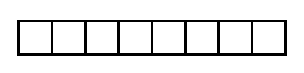
\includegraphics{images/chap2/q29.eps}
\end{figure}

1, 1, 2, 2, 3, 3, 4, 4 ಇವುಗಳನ್ನು ಒಂದು ಮನೆಯಲ್ಲಿ ಒಂದರಂತೆ ತುಂಬಿಸಬೇಕು. ಎರಡು 1ಗಳ ನಡುವೆ ಬೇರೆ ಒಂದು ಅಂಕಿ ಬರಬೇಕು. ಎರಡು 2ಗಳ ನಡುವೆ ಬೇರೆ ಎರಡು ಅಂಕಿ ಬರಬೇಕು. ಎರಡು 3ಗಳ ನಡುವೆ ಬೇರೆ 3 ಅಂಕಿ ಬರಬೇಕು. ಎರಡು 4ಗಳ ನಡುವೆ ಬೇರೆ 4 ಅಂಕಿ ಬರಬೇಕು.

\item ನಾಲ್ಕಂಕಿಯ 4 ಸಂಖ್ಯೆ ಬರೆಯಿರಿ. ಉತ್ತರವನ್ನು ಹಾಳೆಯಲ್ಲಿ ಬರೆದು ಮಡಸಿ ಇಡುತ್ತೇನೆ. ನಿಮ್ಮ ಸಂಖ್ಯೆಯ ಕೆಳಗೆ ನಾನೂ 4 ಅಂಕಿಯ 4 ಸಂಖ್ಯೆ ಬರೆಯುತ್ತೇನೆ. ಕೂಡಿಸಿ ನೋಡಿ. ನಾನು ಬರೆದಿಷ್ಟೇ ಉತ್ತರ ಬರುತ್ತದೆ. 
\end{enumerate}

\smallskip

\begin{center}
\rule{5cm}{1pt}\\[3pt]
{\Large\bfseries ಉತ್ತರಗಳು}\\[-0.1cm]
\rule{5cm}{1pt}
\end{center}

\begin{enumerate}
\itemsep=5pt
\item 
\begin{tabular}[t]{ll}
$1 = \dfrac{44}{44}$ & $6 = \dfrac{4 + 4}{4} + 4$\\[0.3cm]
$2 = \dfrac{4}{4} + \dfrac{4}{4}$ & $7 = 4 + 4 - \dfrac{4}{4}$\\[0.3cm]
$3 = \dfrac{4 + 4 + 4}{4}$ & $8 = 4 + 4 + 4 - 4$\\[0.3cm]
$4 = \dfrac{4 - 4}{4} + 4$ & $9 = 4 + 4 + \dfrac{4}{4}$\\[0.3cm]
$5 = (4 \times 4 + 4) \div 4$ & $10 = \dfrac{44 - 4}{4}$
\end{tabular}

\{ಇದೇ ರೀತಿ 100ರವರಗೆ ಎಲ್ಲಾ ಸಂಖ್ಯೆಗಳನ್ನು ಬರಿಸಬಹುದು ಪ್ರಯತ್ನಿಸಿ \}

\medskip
\item $\dfrac{57429}{06381} = 9 = \dfrac{95742}{10638} = \dfrac{58239}{06471} = \dfrac{75249}{08361}$

\smallskip
\item $98 - 76 + 54 + 3 + 21 = 100$

\item $13 + 3 + 3 + 1 = 20$

\item $173 + 4 = 177,\qquad 85 + 92 = 177$

\item $8 - \dfrac{8}{8} = 7$

\item $XVII \rightarrow \sqrt{\overline{X}} = \sqrt{10000} = 100 \left\{\overline{X} = 10,000\right\}$ ರೋಮನ್ ಸಂಖ್ಯೆಗಳಲ್ಲಿ 

\item $LXVIII \rightarrow \sqrt[4]{\overline{X}} = \sqrt[4]{1000} = 100$

($4$ ಮಾಡಲು $L$ ಮತ್ತು $1$ ಬಳಸಿದೆ)

\item 
\begin{tabular}[t]{ll}
\text{ಎರಡು ಉತ್ತರಗಳಿವೆ} & $IV - III = 1$\\
& $IV - II = II$
\end{tabular}

\item $\dfrac{XXII}{VII} = \Pi$\qquad \{$\dfrac{22}{7} = \Pi$\}

\item $\dfrac{1}{\sqrt{1}} = 1$ \{VII ನಲ್ಲಿ 1 ಗೆರೆಯನ್ನು ಮೇಲೆ ಅಡ್ಡಲಾಗಿ ಬರೆದಿದೆ.\}

\item ಕನಿಷ್ಠ 6 ಕಡ್ಡಿ ತೆಗೆಯಬೇಕು ಕೊಟ್ಟಿರುವುದು

\begin{minipage}[c]{3.5cm}
\begin{figure}[H]
\centering
\includegraphics{images/chap2/q12.eps}
\end{figure}
\end{minipage}
\begin{minipage}[c]{3.5cm}
\begin{figure}[H]
\centering
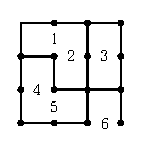
\includegraphics{images/chap2/ans12.eps}
\end{figure}
\end{minipage}
\begin{minipage}[c]{2cm}
ಸಂಖ್ಯೆಗಳ ಸ್ಥಾನದಲ್ಲಿರುವ ಕಡ್ಡಿ ತೆಗೆಯಬೇಕು.
\end{minipage}

\item ಕೊಟ್ಟಿರುವುದು 

\begin{minipage}[c]{4cm}
\begin{figure}[H]
\centering
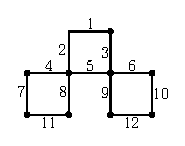
\includegraphics{images/chap2/q13.eps}
\end{figure}
\end{minipage}
\begin{minipage}[c]{5cm}
7, 4, 11 ಸ್ಥಾನ ಪಲ್ಲಟಮಾಡಿದ ನಂತರ
\begin{figure}[H]
\centering
\includegraphics{images/chap2/ans13.eps}
\end{figure}
\end{minipage}

ನಾಲ್ಕು ಚಿಕ್ಕ ಚೌಕಗಳು, 1 ದೊಡ್ಡ ಚೌಕ.

\eject

\item 
~

\begin{minipage}[t]{4cm}
\begin{figure}[H]
\centering
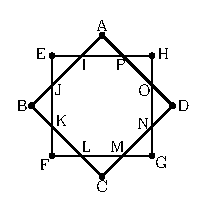
\includegraphics{images/chap2/ans14.eps}
\end{figure}
\end{minipage}
\begin{minipage}[t]{5cm}
\begin{equation*}
\left.
\begin{aligned}
\text{ABCD}\\
\text{EFGH}
\end{aligned}
\right\}
~~  2\text{ ಚೌಕಗಳು}
\end{equation*}
\begin{equation*}
\left.
\begin{aligned}
\text{AIP, BJK, CLM}\\
\text{DNO, EJI, FKL}\\
\text{GMN, HOP}
\end{aligned}
\right\}
~~  8\text{  ತ್ರಿಭುಜಗಳು}
\end{equation*}
IJKLMNOP~  ಬಹುಭುಜಾಕೃತಿ.
\end{minipage}

\item 
~

\begin{figure}[H]
\centering
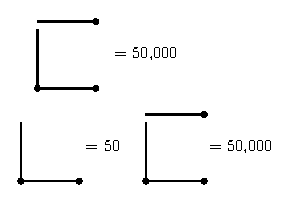
\includegraphics{images/chap2/ans15.eps}
\end{figure}
\{ರೋಮನ್ ಅಂಕಿಗಳ ಮೇಲೆ ಅಡ್ಡಗೀಟು ಎಳೆದರೆ 10,000 ಪಟ್ಟು ಆಗುತ್ತದೆ.\}

\item ಕೊಟ್ಟಿರುವುದು 

\begin{minipage}[c]{5cm}
\begin{figure}[H]
\centering
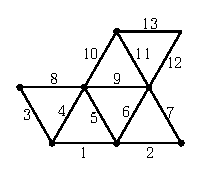
\includegraphics{images/chap2/q16.eps}
\end{figure}
\end{minipage}
\begin{minipage}[c]{4cm}
5, 6, 9 ತೆಗೆದ ನಂತರ 
\begin{figure}[H]
\centering
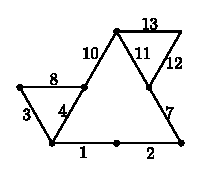
\includegraphics{images/chap2/ans16.eps}
\end{figure}
\end{minipage}

\item 
\begin{tabular}[t]{ccc}
$6666 \times 6666$ & = & $4444 ~355556$\\
$666666 \times 666666$ & = & $44444 ~3555556$\\
$6666666 \times 6666666$ & = & $444444~ 35555556$\\
$66666666 \times 66666666$ & = & $4444444~ 355555556$
\end{tabular}

\item ಉತ್ತರದ ಅಗತ್ಯವಿಲ್ಲ 

\item ಉತ್ತರದ ಅಗತ್ಯವಿಲ್ಲ 

\item 8 ಚೌಕಗಳು 

\begin{minipage}[c]{5cm}
\begin{figure}[H]
\centering
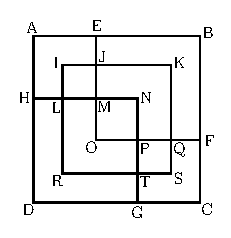
\includegraphics[scale=1.1]{images/chap2/ans20.eps}
\end{figure}
\end{minipage}
\begin{minipage}[c]{4cm}
\begin{tabular}{l}
ABCD\\
EBFO\\
HNED\\
MNOP\\
IJML\\
PQST\\
AEMH\\
PFCG
\end{tabular}
\end{minipage}

\item ಘನಾಕೃತಿಯ ಮೇಲ್ಮೈ ಅಳತೆ ಅದರ 1 ಮುಖದ 6ರಷ್ಟು $x$ ಅಂಗುಲ ಬಾಹುವಿನ ಘನದ ಮೇಲ್ಮೈ $6x^{2}$ ಚ. ಅಂ. ಗಾತ್ರವು ಇಷ್ಟೇ ಅಳತೆ ಎಂದರೆ $x^{3} = 6x^{2}$ ಅಥವಾ $x = 6$

$\therefore 6"$ ಬಾಹುವಿನ ಘನ. ಮೇಲ್ಮೈ $6 \times 6 \times 6$ ಚ. ಅಂ.

ಗಾತ್ರ $6 \times 6 \times 6$ ಘ. ಅಂ.

\item 
~

\begin{minipage}[c]{6cm}
\begin{figure}[H]
\centering
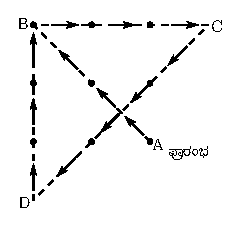
\includegraphics{images/chap2/ans22.eps}
\end{figure}
\end{minipage}
\begin{minipage}[c]{3cm}
\begin{equation*}
\left.
\begin{aligned}
AB\\
BC\\
CD\\
DB
\end{aligned}
\right\}
~~ 4\text{ ಸರಳ ರೇಖೆಗಳು.}
\end{equation*}
\end{minipage}

\item 
~

\begin{figure}[H]
\centering
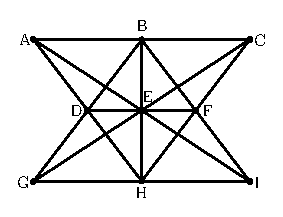
\includegraphics{images/chap2/ans23.eps}
\end{figure}

ABCDEFGHI~ ತೆಂಗಿನ ಸಸಿಗಳು 

\begin{tabular}{lllll}
ADH & BDG & CEG & GHI & \\
AEI & BEH & CEH &  & \text{ ಹತ್ತು ಸಾಲುಗಳು}\\
ABC & BFI & DEF &  & 
\end{tabular}

\item ಎರಡು ವಿಧಾನಗಳಿವೆ

\begin{figure}[H]
\centering
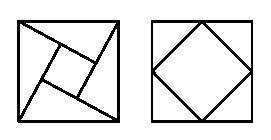
\includegraphics{images/chap2/ans24.eps}
\end{figure}

\item ಒಟ್ಟು ಹೂ $x$ ಇರಲಿ 
\begin{tabbing}
ಪೂಜಿಸಿದ ನಂತರ ಉಳಿಕೆ ~~\= \quad \=  $x - \left(\dfrac{x}{3} + \dfrac{x}{5} + \dfrac{x}{6} + \dfrac{x}{4}\right)$\\[0.1cm]
\quad \> = \> $x - \dfrac{57x}{60} = \dfrac{x}{20}$\\
~~~\quad $\dfrac{x}{20} = 6$ ~ ~$\therefore~ x$ \> = \> $120$\\
\> \> $120$~ ಹೂ
\end{tabbing}

\smallskip
ಅಂಕಗಣಿತ ವಿಧಾನ 

ಒಟ್ಟು ಹೂ 1 ಇರಲಿ 

ನಾಲ್ಕು ದೇವರನ್ನು ಪೂಜಿಸಿದ ನಂತರ ಉಳಿಕೆ $1 - \left(\dfrac{1}{3} + \dfrac{1}{5} + \dfrac{1}{6} + \dfrac{1}{4}\right)$

\begin{align*}
& = 1 - \dfrac{20 + 12 + 10 + 15}{60} = 1 - \dfrac{57}{60}\\
& = 1 - \dfrac{19}{20} = \dfrac{1}{20}
\end{align*}

ಉಳಿಕೆ $\frac{1}{20}$ ಆದರೆ ಒಟ್ಟು ಹೂ 1

6 ಆದರೆ ಒಟ್ಟು ಹೂ 20 $\times$ 6 = 120

\item 
~
\begin{minipage}[t]{4cm}
AB ಕಂಭವಿರಲಿ 9 ಮೊಳ 

AD = 27 ಮೊಳ 
\end{minipage}
\begin{minipage}[t]{5cm}
\begin{figure}[H]
\centering
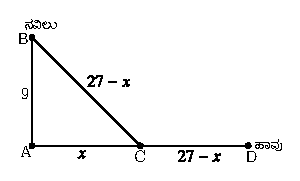
\includegraphics{images/chap2/ans26.eps}
\end{figure}
\end{minipage}

\smallskip
C ಯಲ್ಲಿ  ನವಿಲು ಹಾವನ್ನು ಹಿಡಿಯುತ್ತದೆಂದು ಭಾವಿಸೋಣ.

AC = x ಆದರೆ, \qquad CD = 27 - x = BC

ABC ತ್ರಿಭುಜದಿಂದ \qquad $x^{2} + 9^{2} = (27 - x)^{2}$
\begin{align*}
x^{2} + 81 & = 729 - 54x + x^{2}\\
\therefore\quad 54x & = 729 - 81\\
54x & = 648\\
x & = 12 ~\text{ ಹಸ್ತಗಳು}
\end{align*}

\item 1 ಒಬ್ಬನೇ ರಾಮೇಗೌಡ 

\item 
~

\begin{figure}[H]
\centering
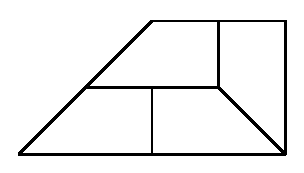
\includegraphics{images/chap2/ans28.eps}
\end{figure}

\item 
~

\begin{figure}[H]
\centering
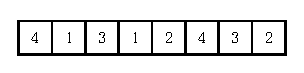
\includegraphics{images/chap2/ans29.eps}
\end{figure}

\eject

\item ಯಾವಾಗಲೂ ಉತ್ತರ 39996

ನಾನು ಬರೆಯುವ ಸಂಖ್ಯೆಗಳು ಅವರು ಬರೆದ ಸಂಖ್ಯೆಗಳ 9ರ ಪೂರಕ 

\begin{minipage}[c]{5cm}
\begin{tabular}[t]{lll}
{\bf ಉದಾ:} & 
$
\left.
\begin{aligned}
& 4327 \\[-0.2cm]
& 5461 \\[-0.2cm]
& 8032 \\[-0.2cm]
& 7253 \\[5pt]
\end{aligned}
\right\}$
\quad ಅವರದ್ದು\\[0.4cm]
&
$
\left.
\begin{aligned}
& 5672\\[-0.2cm]
& 4538\\[-0.2cm]
& 1967\\[-0.2cm]
& 2746
\end{aligned}
\right\}$
\quad ನನ್ನವು\\\hline
& $39996$
\end{tabular}
\end{minipage}
\begin{minipage}[c]{4cm}
\begin{tabular}{l}
4327\\
5672\\
\hline
9999
\end{tabular}
\end{minipage}
\end{enumerate}
